% Search for all the places that say "PUT SOMETHING HERE".

\documentclass[11pt]{article}
\usepackage{amsmath,textcomp,amssymb,graphicx,enumerate,hyperref,enumitem,mathtools,tikz-qtree,listings,chemformula,bm,graphicx,grffile,gensymb,physics,amssymb}
\graphicspath{{/Users/jonathansun5/Documents/Fall 2017/MCB 166/Homeworks/HW 2/Screen Shot 2017-10-02 at 2.51.29 AM.png}{/Users/jonathansun5/Documents/Fall 2017/MCB 166/Homeworks/HW 2/Screen Shot 2017-10-03 at 5.27.43 AM.png}{/Users/jonathansun5/Documents/Fall 2017/MCB 166/Homeworks/HW 2/Screen Shot 2017-10-03 at 5.59.34 AM.png}}

\makeatletter
\newcommand{\leqnos}{\tagsleft@true\let\veqno\@@leqno}
\newcommand{\reqnos}{\tagsleft@false\let\veqno\@@eqno}
\reqnos
\makeatother

\def\Name{Jonathan Sun}  % Your name
\def\SID{25020651}  % Your student ID number
\def\Homework{2} % Number of Homework
\def\Session{Fall 2017}


\title{MCB166 --- \Session --- Problem Set \Homework}
\author{\Name, SID \SID}
\markboth{MCB166 --- \Session --- Problem Set \Homework --- \Name}{MCB166 --- \Session --- Problem Set \Homework --- \Name}
\pagestyle{myheadings}
\date{}

\def\endproofmark{$\Box$}
\newenvironment{proof}{\par{\bf Proof:}}{\endproofmark\smallskip}

\usepackage[margin=1in]{geometry}



\begin{document}
\maketitle

\newpage
\begin{enumerate}[label=\arabic*.]
\item
\underline{Threshold-switch model of excitation}
\vspace*{1\baselineskip}
\\
A resting membrane is mainly potassium selective with a resting membrane potential $E_r = -70 \text{mV}$. The membrane is stimulated by steps of constant current. When the membrane potential is depolarized to a threshold voltage, $\left(V\text{*} = -50 \text{mV}\right)$, a large $\ch{Na}$ conductance is switched on, so that the membrane equilibrium potential is now near the $\ch{Na}$ reversal potential, $E_{\ch{Na}} = +50\text{mV}$. Say that $G_r = 10^{-6} \text{mho}$, $G_{\ch{Na}} = 10^{-4} \text{mho}$, $C = 10^{-9} \text{farads}$.
\vspace*{1\baselineskip}
\\
The voltage follows the differential equation
\begin{align*}
I = C \frac{dV} {dt} + G_{\ch{K}} \left(V - V_{\ch{K}}\right) + S \left(V - V\text{*}\right) G_{\ch{Na}} \left(V - V_{\ch{Na}}\right),
\end{align*}
where $S \left(V - V\text{*}\right)$ is a step function of voltage centered about threshold, $S(x) = 0$ for $x < 0$, $S(x) = 1$ for $x > 0$. This is a nicer way to write the pair of equations we did in class.
\begin{enumerate}[label=(\alph*)]
\item
Solve for the voltage for $3$ different values of stimulus, $I = 0.5 I_{Rh}$, $1.5 I_{Rh}$, and $2 I_{Rh}$.
\vspace*{1\baselineskip}
\\
Here $I_{Rh} = G_r \left(V\text{*} - E_r\right) = 2 \times 10^{-8} \text{amp}$ is the minimum current needed to reach threshold. Use $t^{\text{*}}$ as the time when $V(t)$ reaches $V^{\text{*}}$. Recall that both equations (above and below threshold) have solutions of the form $V(t) = A + B e^{-ct}$, where $A$, $B$, and $c$ are obtained from the initial and steady-state conditions for each solution and one switches equations at $t = t^{\text{*}}$ which becomes the initial time for the `excited' phase. Plot the three solutions on the same $V$-$t$ graph.
\vspace*{1\baselineskip}
\\
To solve this problem, we first notice that $S(x) = 0$ for $x < 0$, $S(x) = 1$ for $x > 0$. In other words, we get this:
\begin{align*}
S (V - V\text{*}) = \left\{
\begin{array}{ll}
	0 & \text{for } V - V\text{*} < 0 \rightarrow V < V\text{*} \\
	1 & \text{for } V - V\text{*} > 0 \rightarrow V > V\text{*} \\
\end{array}
\right.
\end{align*}
This gives us:
\begin{align*}
I = \left\{
\begin{array}{ll}
	C \frac{dV} {dt} + G_{\ch{K}} \left(V - E_{\ch{K}}\right) & \text{for } V < V\text{*} \\
	C \frac{dV} {dt} + G_{\ch{K}} \left(V - E_{\ch{K}}\right) + G_{\ch{Na}} \left(V - E_{\ch{Na}}\right) & \text{for } V > V\text{*} \\
\end{array}
\right.
\end{align*}
I will first solve for the first equation when $V < V\text{*}$ and then solve for the second equation when $V > V\text{*}$.
\vspace*{1\baselineskip}
\\
For Eqn(1) when $V < V\text{*}$:
\begin{align*}
I = C \frac{dV} {dt} + G_{\ch{K}} \left(V - E_{\ch{K}}\right)
\end{align*}
\begin{align*}
C \frac{dV} {dt} + G_{\ch{K}} V = I + G_{\ch{K}} E_{\ch{K}}
\end{align*}
\begin{align*}
\frac{dV} {dt} + \frac{G_{\ch{K}}} {C} V = \frac{I + G_{\ch{K}} E_{\ch{K}}} {C}
\end{align*}
Using the method of integrating factors, we know that an equation of:
\begin{align*}
\frac{dV} {dt} + p V = q
\end{align*}
Will yield:
\begin{align*}
V(t) = e^{-pt} q \int e^{pt} \mathrm{d}t = e^{-pt} q \left[\frac{e^{pt}} {p} + D_1\right]
\end{align*}
So, with our $p = \frac{G_{\ch{K}}} {C}$ and $q = \frac{I + G_{\ch{K}} E_{\ch{K}}} {C}$, we get the following:
\begin{align*}
V(t) = e^{-\frac{G_{\ch{K}}} {C} t} \times \frac{I + G_{\ch{K}} E_{\ch{K}}} {C} \times \left[\frac{e^{\frac{G_{\ch{K}}} {C} t}} {\frac{G_{\ch{K}}} {C}} + D_1\right]
\end{align*}
\begin{align*}
V(t) = e^{-\frac{G_{\ch{K}}} {C} t} \times \frac{I + G_{\ch{K}} E_{\ch{K}}} {C} \times \left[\frac{C} {G_{\ch{K}}} e^{\frac{G_{\ch{K}}} {C} t} + D_1\right]
\end{align*}
Since $V(t = 0) = \text{resting membrane potential} = -70 \text{mV} = E_{\ch{K}}$:
\begin{align*}
V(0) = \frac{I + G_{\ch{K}} E_{\ch{K}}} {C} \times \left[\frac{C} {G_{\ch{K}}} + D_1\right] = E_{\ch{K}}
\end{align*}
\begin{align*}
\frac{C} {G_{\ch{K}}} + D_1 =  \frac{E_{\ch{K}}C} {I + G_{\ch{K}} E_{\ch{K}}}
\end{align*}
\begin{align*}
D_1 =  \frac{E_{\ch{K}}C} {I + G_{\ch{K}} E_{\ch{K}}} - \frac{C} {G_{\ch{K}}}
\end{align*}
Thus, the equation is:
\begin{align*}
V(t) = e^{-\frac{G_{\ch{K}}} {C} t} \times \frac{I + G_{\ch{K}} E_{\ch{K}}} {C} \times \left[\frac{C} {G_{\ch{K}}} e^{\frac{G_{\ch{K}}} {C} t} + \frac{E_{\ch{K}}C} {I + G_{\ch{K}} E_{\ch{K}}} - \frac{C} {G_{\ch{K}}}\right]
\end{align*}
\begin{align*}
V(t) = \frac{I + G_{\ch{K}} E_{\ch{K}}} {G_{\ch{K}}} + E_{\ch{K}} e^{-\frac{G_{\ch{K}}} {C} t} - \frac{I + G_{\ch{K}} E_{\ch{K}}} {G_{\ch{K}}} e^{-\frac{G_{\ch{K}}} {C} t}
\end{align*}
\begin{align*}
V(t) = \frac{I} {G_{\ch{K}}} + E_{\ch{K}} + E_{\ch{K}} e^{-\frac{G_{\ch{K}}} {C} t} - \frac{I} {G_{\ch{K}}} e^{-\frac{G_{\ch{K}}} {C} t} - E_{\ch{K}} e^{-\frac{G_{\ch{K}}} {C} t}
\end{align*}
\begin{align*}
V(t) = \frac{I} {G_{\ch{K}}} + E_{\ch{K}} - \frac{I} {G_{\ch{K}}} e^{-\frac{G_{\ch{K}}} {C} t}
\end{align*}
\begin{align*}
V(t) = E_{\ch{K}} + \frac{I} {G_{\ch{K}}} \left(1 - e^{-\frac{G_{\ch{K}}} {C} t}\right)
\end{align*}
Thus, we get $V(t) = E_{\ch{K}} + \frac{I} {G_{\ch{K}}} \left(1 - e^{-\frac{G_{\ch{K}}} {C} t}\right)$ for $V < V\text{*}$.
\vspace*{1\baselineskip}
\\
For Eqn(2) when $V > V\text{*}$:
\begin{align*}
I = C \frac{dV} {dt} + G_{\ch{K}} \left(V - E_{\ch{K}}\right) + G_{\ch{Na}} \left(V - E_{\ch{Na}}\right)
\end{align*}
\begin{align*}
C \frac{dV} {dt} + G_{\ch{K}} V + G_{\ch{Na}} V = I + G_{\ch{K}} E_{\ch{K}} + G_{\ch{Na}} E_{\ch{Na}}
\end{align*}
\begin{align*}
\frac{dV} {dt} + \frac{G_{\ch{K}} + G_{\ch{Na}}} {C} V = \frac{I + G_{\ch{K}} E_{\ch{K}} + G_{\ch{Na}} E_{\ch{Na}}} {C}
\end{align*}
Using the method of integrating factors, we know that an equation of:
\begin{align*}
\frac{dV} {dt} + p V = q
\end{align*}
Will yield:
\begin{align*}
V(t) = e^{-pt} q \int e^{pt} \mathrm{d}t = e^{-pt} q \left[\frac{e^{pt}} {p} + D_2\right]
\end{align*}
So, with our $p = \frac{G_{\ch{K}} + G_{\ch{Na}}} {C}$ and $q = \frac{I + G_{\ch{K}} E_{\ch{K}} + G_{\ch{Na}} E_{\ch{Na}}} {C}$, we get the following:
\begin{align*}
V(t) = e^{-pt} q \left[\frac{e^{pt}} {p} + D_2\right]
\end{align*}
Since our initial condition is $V(t = t\text{*}) = V\text{*}$:
\begin{align*}
V\text{*} = e^{-pt\text{*}} q \left[\frac{e^{pt\text{*}}} {p} + D_2\right]
\end{align*}
\begin{align*}
V\text{*} = \frac{q} {p} + D_2 \times q e^{-pt\text{*}}
\end{align*}
\begin{align*}
D_2 \times q e^{-pt\text{*}} = V\text{*} - \frac{q} {p}
\end{align*}
\begin{align*}
D_2 = \frac{V\text{*}} {q e^{-pt\text{*}}} - \frac{1} {p e^{-pt\text{*}}}
\end{align*}
Thus, the equation is:
\begin{align*}
V(t) = e^{-pt} q \left[\frac{e^{pt}} {p} + \frac{V\text{*}} {q e^{-pt\text{*}}} - \frac{1} {p e^{-pt\text{*}}}\right]
\end{align*}
\begin{align*}
V(t) = \frac{q} {p} + \frac{e^{-pt} V\text{*}} {e^{-pt\text{*}}} - \frac{q e^{-pt}} {p e^{-pt\text{*}}}
\end{align*}
\begin{align*}
V(t) = \frac{q} {p} + e^{-p\left(t - t\text{*}\right)} V\text{*} - \frac{q} {p} e^{-p\left(t - t\text{*}\right)}
\end{align*}
\begin{align*}
V(t) = V\text{*} + \frac{q} {p} - \frac{q} {p} e^{-p\left(t - t\text{*}\right)} - V\text{*} + e^{-p\left(t - t\text{*}\right)} V\text{*}
\end{align*}
\begin{align*}
V(t) = V\text{*} + \frac{q} {p} \left(1 - e^{-p\left(t - t\text{*}\right)}\right) - V\text{*} \left(1 - e^{-p\left(t - t\text{*}\right)}\right)
\end{align*}
\begin{align*}
V(t) = V\text{*} + \left(\frac{q} {p} - V\text{*}\right) \left(1 - e^{-p\left(t - t\text{*}\right)}\right)
\end{align*}
Thus, we get $V(t) = V\text{*} + \left(\frac{q} {p} - V\text{*}\right) \left(1 - e^{-p\left(t - t\text{*}\right)}\right)$ for $V > V\text{*}$ where $p = \frac{G_{\ch{K}} + G_{\ch{Na}}} {C}$ and $q = \frac{I + G_{\ch{K}} E_{\ch{K}} + G_{\ch{Na}} E_{\ch{Na}}} {C}$.
\vspace*{1\baselineskip}
\\
To solve for $t\text{*}$, or time where the two equations intersect I will solve for the first equation with respect to time $t = t\text{*}$:
\begin{align*}
V(t) = E_{\ch{K}} + \frac{I} {G_{\ch{K}}} \left(1 - e^{-\frac{G_{\ch{K}}} {C} t}\right)
\end{align*}
\begin{align*}
V(t\text{*}) = V\text{*} = E_{\ch{K}} + \frac{I} {G_{\ch{K}}} \left(1 - e^{-\frac{G_{\ch{K}}} {C} t\text{*}}\right)
\end{align*}
Since it is given that $V\text{*} = -50 \text{mV} = -0.05 \text{V}$, $E_{\ch{K}} = -70 \text{mV} = -0.07 \text{V}$, $G_r = 10^{-6} \text{mho}$, and $C = 10^{-9} \text{farads}$:
\begin{align*}
-0.05 = -0.07 + \frac{I} {10^{-6}} \left(1 - e^{-\frac{10^{-6}} {10^{-9}} t\text{*}}\right)
\end{align*}
\begin{align*}
0.02 = \frac{I} {10^{-6}} \left(1 - e^{-\frac{10^{-6}} {10^{-9}} t\text{*}}\right)
\end{align*}
\begin{align*}
2 \times 10^{-8} = I \left(1 - e^{-1000 t\text{*}}\right)
\end{align*}
\begin{align*}
\frac{2 \times 10^{-8}} {I} = 1 - e^{-1000 t\text{*}}
\end{align*}
We can solve for $t\text{*}$ when $I = 0.5 I_{Rh}$, $1.5 I_{Rh}$, and $2 I_{Rh}$, with $I_{Rh} = 2 \times 10^{-8} \text{amp}$:
\vspace*{1\baselineskip}
\\
When $I = 0.5 I_{Rh}$, $I = 10^{-8} \text{amp}$:
\begin{align*}
\frac{2 \times 10^{-8}} {10^{-8}} = 1 - e^{-1000 t\text{*}}
\end{align*}
\begin{align*}
2 = 1 - e^{-1000 t\text{*}}
\end{align*}
\begin{align*}
-1 = e^{-1000 t\text{*}}
\end{align*}
This gives an imaginary number when I solve for $t\text{*}$, which makes sense since it has not reached the minimum current needed.
\vspace*{1\baselineskip}
\\
When $I = 1.5 I_{Rh}$, $I = 3 \times 10^{-8} \text{amp}$:
\begin{align*}
\frac{2 \times 10^{-8}} {3 \times 10^{-8}} = 1 - e^{-1000 t\text{*}}
\end{align*}
\begin{align*}
\frac{2} {3} = 1 - e^{-1000 t\text{*}}
\end{align*}
\begin{align*}
\frac{1} {3} = e^{-1000 t\text{*}}
\end{align*}
\begin{align*}
\ln{\frac{1} {3}} = \ln{e^{-1000 t\text{*}}}
\end{align*}
\begin{align*}
\ln{\frac{1} {3}} = -1000 t\text{*}
\end{align*}
\begin{align*}
t\text{*} = - \frac{1} {1000} \ln{\frac{1} {3}}
\end{align*}
\begin{align*}
t\text{*} \approx 0.0011
\end{align*}
This means that when $I = 1.5 I_{Rh} = 3 \times 10^{-8} \text{amp}$, it will take approximately $0.0011$ seconds to reach the threshold.
\vspace*{1\baselineskip}
\\
When $I = 2 I_{Rh}$, $I = 4 \times 10^{-8} \text{amp}$:
\begin{align*}
\frac{2 \times 10^{-8}} {4 \times 10^{-8}} = 1 - e^{-1000 t\text{*}}
\end{align*}
\begin{align*}
\frac{1} {2} = 1 - e^{-1000 t\text{*}}
\end{align*}
\begin{align*}
\frac{1} {2} = e^{-1000 t\text{*}}
\end{align*}
\begin{align*}
\ln{\frac{1} {2}} = \ln{e^{-1000 t\text{*}}}
\end{align*}
\begin{align*}
\ln{\frac{1} {2}} = -1000 t\text{*}
\end{align*}
\begin{align*}
t\text{*} = - \frac{1} {1000} \ln{\frac{1} {2}}
\end{align*}
\begin{align*}
t\text{*} \approx 6.9315 \times 10^{-4}
\end{align*}
This means that when $I = 2 I_{Rh} = 4 \times 10^{-8} \text{amp}$, it will take approximately $6.9315 \times 10^{-4}$ or $0.00069315$ seconds to reach the threshold.
\vspace*{1\baselineskip}
\\
The graph ends up looking like this:
\begin{center}
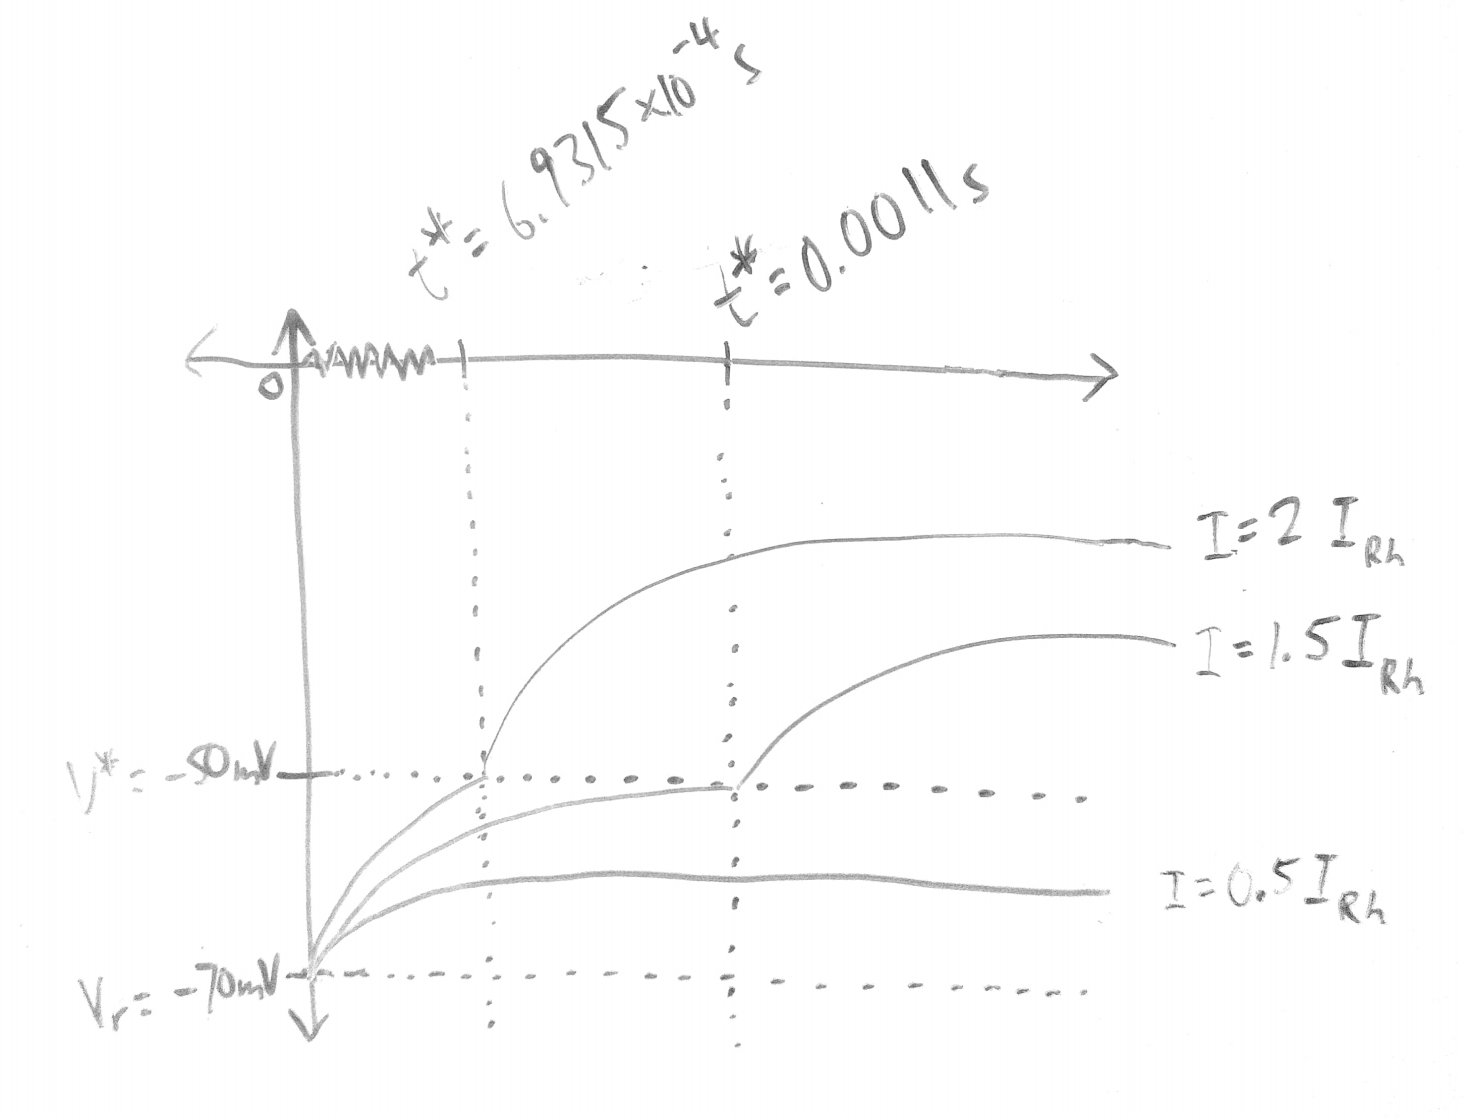
\includegraphics[width=0.75\textwidth]{/Users/jonathansun5/Documents/Fall 2017/MCB 166/Homeworks/HW 2/Screen Shot 2017-10-03 at 5.27.43 AM.png}
\end{center}



\newpage
\item
Plot the steady state current-voltage relation under constant voltage (voltage-clamp) conditions (ie. the current voltage relation obtained by setting $dV / dt = 0$).
\vspace*{1\baselineskip}
\\
To solve this problem, we will use the current equations from part a:
\begin{align*}
I = \left\{
\begin{array}{ll}
	C \frac{dV} {dt} + G_{\ch{K}} \left(V - E_{\ch{K}}\right) & \text{for } V < V\text{*} \\
	C \frac{dV} {dt} + G_{\ch{K}} \left(V - E_{\ch{K}}\right) + G_{\ch{Na}} \left(V - E_{\ch{Na}}\right) & \text{for } V > V\text{*} \\
\end{array}
\right.
\end{align*}
Since $\frac{dV} {dt} = 0$ we get:
\begin{align*}
I = \left\{
\begin{array}{ll}
	G_{\ch{K}} \left(V - E_{\ch{K}}\right) & \text{for } V < V\text{*} \\
	G_{\ch{K}} \left(V - E_{\ch{K}}\right) + G_{\ch{Na}} \left(V - E_{\ch{Na}}\right) & \text{for } V > V\text{*} \\
\end{array}
\right.
\end{align*}
When $V < V\text{*}$:
\begin{align*}
I = G_{\ch{K}} \left(V - E_{\ch{K}}\right)
\end{align*}
\begin{align*}
I = 10^{-6} \left(-0.07 + 0.07\right)
\end{align*}
\begin{align*}
I = 0
\end{align*}
Thus, the current is $0$ amps when $V < V\text{*}$.
When $V > V\text{*}$:
\begin{align*}
I = G_{\ch{K}} \left(V - E_{\ch{K}}\right) + G_{\ch{Na}} \left(V - E_{\ch{Na}}\right)
\end{align*}
\begin{align*}
I = 10^{-6} \left(-0.05 + 0.07\right) + 10^{-4} \left(-0.05 + 0.05\right)
\end{align*}
\begin{align*}
I = 10^{-6} \left(0.02\right)
\end{align*}
\begin{align*}
I = 2 \times 10^{-8}
\end{align*}
Thus, the current is $2 \times 10^{-8}$ amps when $V > V\text{*}$.
\vspace*{1\baselineskip}
\\
The graph ends up looking like this:
\begin{center}
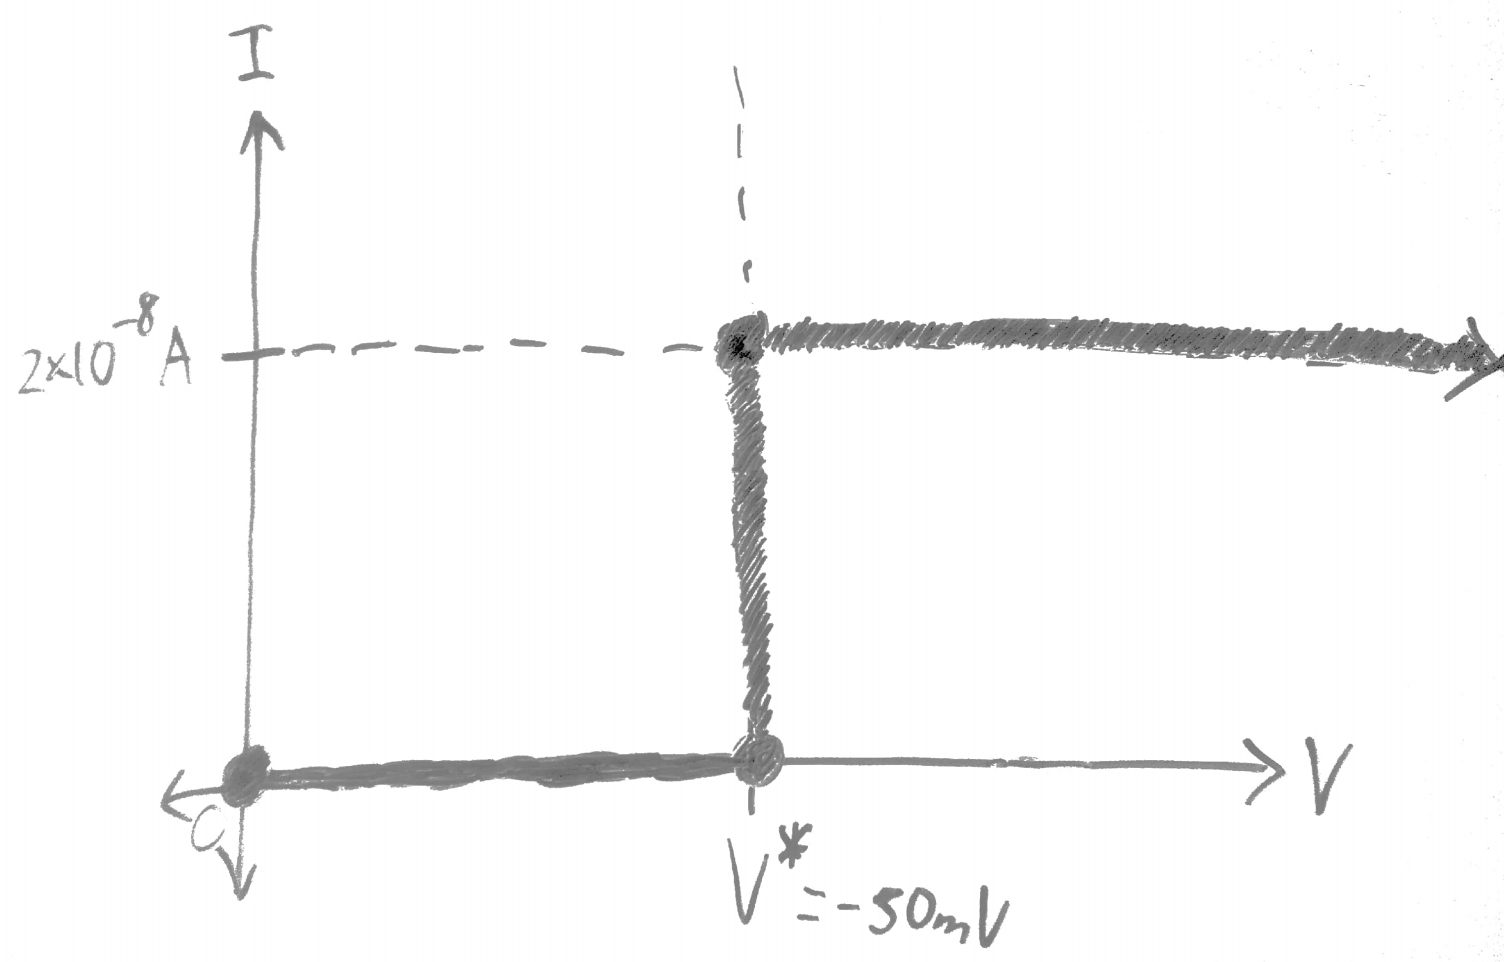
\includegraphics[width=0.75\textwidth]{/Users/jonathansun5/Documents/Fall 2017/MCB 166/Homeworks/HW 2/Screen Shot 2017-10-03 at 5.59.34 AM.png}
\end{center}
\end{enumerate}



\newpage
\item
\underline{Strength-Duration Relation} (Lapique's Law)
\vspace*{1\baselineskip}
\\
For constant-current stimuli, the amplitude and duration of the stimulating current step are related by Lapique's Law,
\begin{align*}
I\text{*} = I_{Rh} / (1 - \text{exp}(-t\text{*} / T))
\end{align*}
$I_{Rh}$, called the rheobase is the minimum current which can cause excitation. T is the membrane the characteristic membrane time constant.
\vspace*{1\baselineskip}
\\
Using the current-clamp response to the different current steps (ie. the results of prob. 1), derive Lapique's law (ie. calculate the time it takes for the voltage to reach V\text{*} as a function of stimulus amplitude, I\text{*} and the time to reach threshold for that particular stimulus, t\text{*}).
\vspace*{1\baselineskip}
\\
To solve this problem, we start with:
\begin{align*}
V(t_\theta) = V_\theta = E_r + \frac{I} {G_r} \left(1 - e ^ {\frac{-t_\theta} {\tau}}\right)
\end{align*}
Which I will rewrite as:
\begin{align*}
V\text{*} = E_r + \frac{I\text{*}} {G_r} \left(1 - e ^ {\frac{-t\text{*}} {T}}\right)
\end{align*}
\begin{align*}
V\text{*} - E_r = \frac{I\text{*}} {G_r} \left(1 - e ^ {\frac{-t\text{*}} {T}}\right)
\end{align*}
\begin{align*}
G_r \left(V\text{*} - E_r\right) = I\text{*} \left(1 - e ^ {\frac{-t\text{*}} {T}}\right)
\end{align*}
From problem 1, we were given that:
\begin{align*}
I_{Rh} = G_r \left(V\text{*} - E_r\right)
\end{align*}
Therefore, we can rewrite the equation as:
\begin{align*}
I_{Rh} = I\text{*} \left(1 - e ^ {\frac{-t\text{*}} {T}}\right)
\end{align*}
\begin{align*}
I\text{*} = \frac{I_{Rh}} {1 - e ^ {\frac{-t\text{*}} {T}}}
\end{align*}
Therefore, we have derived Lapique's law using the current-clamp response to different current steps.



\newpage
\item
\underline{Equivalent Circuit with Electrogenic Pump}
\begin{center}
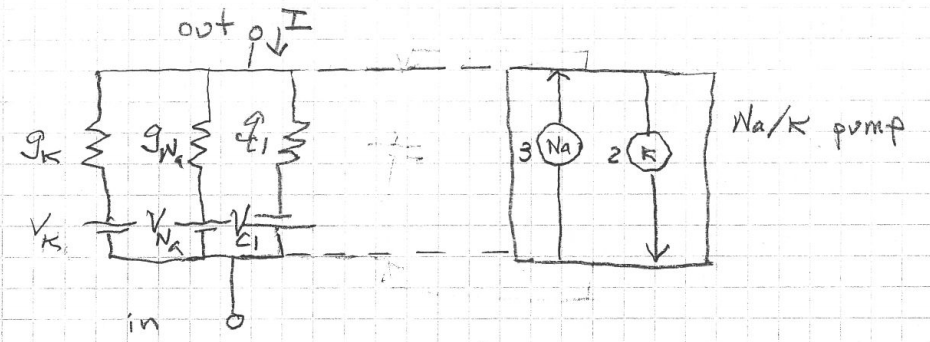
\includegraphics[width=1\textwidth]{/Users/jonathansun5/Documents/Fall 2017/MCB 166/Homeworks/HW 2/Screen Shot 2017-10-02 at 2.51.29 AM.png}
\end{center}
The figure shows the equivalent circuit for an axon at rest in parallel with an equivalent constant-current source representing the \ch{Na+}/\ch{K+}-ATPase pump.
\begin{enumerate}[label=(\alph*)]
\item
Write an expression for the reversal potential (in the absence of the pump) in terms of $V_{\ch{K}}$, $V_{\ch{Na}}$, $V_{\ch{Cl}}$ and the \underline{relative} conductances
\begin{align*}
\alpha = g_{\ch{Na}} / g_{\ch{K}} \text{ and } \beta = g_{\ch{Cl}} / g_{\ch{K}}.
\end{align*}
Is this situation, $I_{\ch{L}} = I_{\ch{K}} + I_{\ch{Na}} + I_{\ch{Cl}} = 0$, an equilibrium? If not, why not?
\vspace*{1\baselineskip}
\\
To solve this problem, we start with:
\begin{align*}
I_{total} = G_{\ch{K}} \left(V_r - E_{\ch{K}}\right) + G_{\ch{Na}} \left(V_r - E_{\ch{Na}}\right) + G_{\ch{Cl}} \left(V_r - E_{\ch{Cl}}\right) = 0
\end{align*}
\begin{align*}
G_{\ch{K}} V_r - G_{\ch{K}} E_{\ch{K}} + G_{\ch{Na}} V_r - G_{\ch{Na}} E_{\ch{Na}} + G_{\ch{Cl}} V_r - G_{\ch{Cl}} E_{\ch{Cl}} = 0
\end{align*}
\begin{align*}
G_{\ch{K}} V_r + G_{\ch{Na}} V_r + G_{\ch{Cl}} V_r = G_{\ch{K}} E_{\ch{K}} + G_{\ch{Na}} E_{\ch{Na}} + G_{\ch{Cl}} E_{\ch{Cl}}
\end{align*}
Dividing both sides by $G_{\ch{K}}$ gives us:
\begin{align*}
\frac{G_{\ch{K}} V_r + G_{\ch{Na}} V_r + G_{\ch{Cl}} V_r} {G_{\ch{K}}} = \frac {G_{\ch{K}} E_{\ch{K}} + G_{\ch{Na}} E_{\ch{Na}} + G_{\ch{Cl}} E_{\ch{Cl}}} {G_{\ch{K}}}
\end{align*}
\begin{align*}
V_r + \frac{G_{\ch{Na}}} {G_{\ch{K}}} V_r + \frac{G_{\ch{Cl}}} {G_{\ch{K}}} V_r = E_{\ch{K}} + \frac{G_{\ch{Na}}} {G_{\ch{K}}} E_{\ch{Na}} + \frac{G_{\ch{Cl}}} {G_{\ch{K}}} E_{\ch{Cl}}
\end{align*}
Substituting in $\alpha = \frac{g_{\ch{Na}}} {g_{\ch{K}}}$ and $\beta = \frac {g_{\ch{Cl}}} {g_{\ch{K}}}$ gives us:
\begin{align*}
V_r + \alpha V_r + \beta V_r = E_{\ch{K}} + \alpha E_{\ch{Na}} + \beta E_{\ch{Cl}}
\end{align*}
\begin{align*}
V_r = \frac{E_{\ch{K}} + \alpha E_{\ch{Na}} + \beta E_{\ch{Cl}}} {1 + \alpha + \beta} = \frac{G_{\ch{K}} E_{\ch{K}} + G_{\ch{Na}} E_{\ch{Na}} + G_{\ch{Cl}} E_{\ch{Cl}}} {G_{\ch{K}} + G_{\ch{Na}} + G_{\ch{Cl}}}
\end{align*}
The situation, $I_{\ch{L}} = I_{\ch{K}} + I_{\ch{Na}} + I_{\ch{Cl}} = 0$, is not in equilibrium because although the total current is $0$, each ion's currents are not at equilibrium.



\newpage
\item
Now introduce the pump
\begin{align*}
I_{pump} = I_{\ch{Na}-pump} + I_{\ch{K}-pump},
\end{align*}
\begin{align*}
I_{\ch{Na}-pump} =  -\frac{3} {2} I_{\ch{K}-pump}.
\end{align*}
Write the expression for the new resting potential in terms of the batteries and (new) \underline{relative} permeabilities. Use the equilibrium conditions:
\begin{align*}
I_{\ch{Na}} = I_{\ch{Na}-leak} + I_{\ch{Na}-pump}
\end{align*}
\begin{align*}
I_{\ch{K}} = I_{\ch{K}-leak} + I_{\ch{K}-pump},
\end{align*}
\begin{align*}
I_{\ch{Cl}} = 0
\end{align*}
To solve this problem, we start with:
\begin{align*}
I_{pump} = I_{\ch{Na}-pump} + I_{\ch{K}-pump}
\end{align*}
\begin{align*}
I_{pump} = I_{\ch{Na}-leak} + I_{\ch{Na}-pump} + I_{\ch{K}-leak} + I_{\ch{K}-pump} = 0
\end{align*}
\begin{align*}
I_{\ch{Na}-leak} + \left(-\frac{3} {2} I_{\ch{K}-pump}\right) + I_{\ch{K}-leak} + I_{\ch{K}-pump} = 0
\end{align*}
\begin{align*}
I_{\ch{Na}-leak} - \frac{1} {2} I_{\ch{K}-pump} + I_{\ch{K}-leak} = 0
\end{align*}
\begin{align*}
I_{\ch{Na}-leak} + \frac{1} {2} I_{\ch{K}-leak} + I_{\ch{K}-leak} = 0
\end{align*}
\begin{align*}
I_{\ch{Na}-leak} + \frac{3} {2} I_{\ch{K}-leak} = 0
\end{align*}
This equation can be rewritten as:
\begin{align*}
G_{\ch{Na}} \left(V_r - E_{\ch{Na}}\right) + \frac{3} {2} G_{\ch{K}} \left(V_r - E_{\ch{K}}\right) = 0
\end{align*}
\begin{align*}
G_{\ch{Na}} V_r - G_{\ch{Na}} E_{\ch{Na}} + \frac{3} {2} G_{\ch{K}} V_r - \frac{3} {2} G_{\ch{K}} E_{\ch{K}} = 0
\end{align*}
\begin{align*}
G_{\ch{Na}} V_r + \frac{3} {2} G_{\ch{K}} V_r = G_{\ch{Na}} E_{\ch{Na}} + \frac{3} {2} G_{\ch{K}} E_{\ch{K}}
\end{align*}
\begin{align*}
V_r = \frac{G_{\ch{Na}} E_{\ch{Na}} + \frac{3} {2} G_{\ch{K}} E_{\ch{K}}} {G_{\ch{Na}} + \frac{3} {2} G_{\ch{K}}}
\end{align*}



\newpage
\item
Show that the formula you derived is still valid when you ignore the chloride terms (as I did in the worked example\text{*}). Explain this by working out the relation between the equilibrium concentrations of \ch{Cl-} and the membrane potential.
\vspace*{1\baselineskip}
\\
To solve this problem, we start with:
\begin{align*}
I_{\ch{Cl}} = 0
\end{align*}
This equation can be rewritten as:
\begin{align*}
G_{\ch{Cl}} \left(V_r - E_{\ch{Cl}}\right) = 0
\end{align*}
Dividing both sides by $G_{\ch{Cl}}$ gives us:
\begin{align*}
\frac{G_{\ch{Cl}} \left(V_r - E_{\ch{Cl}}\right)} {G_{\ch{Cl}}} = \frac{0} {G_{\ch{Cl}}}
\end{align*}
\begin{align*}
V_r - E_{\ch{Cl}} = 0
\end{align*}
\begin{align*}
V_r = E_{\ch{Cl}}
\end{align*}
Since $V_r = E_{\ch{Cl}}$, this means that the reversal potential is equal to the equilibrium potential for chloride. Since chloride's equilibrium potential matches the reversal potential, there is essentially no net flow for chloride and therefore we can just ignore chloride.
\end{enumerate}



\end{enumerate}
\end{document}
